%%%%%%%%%%%%%%%%%%%%%%%%%%%%%%%%
\section{Overview}
\label{sec:detectors-fd-ref-ov}


This chapter describes the reference design of the DUNE far detector.
The reference design consists of four nominal \ktadj{10} fiducial
mass, single-phase LArTPC modules, augmented with photon detection
systems.  A ``single-phase'' detector is one in which the charge
generation, drift and collection all occur in liquid argon (LAr). The
scope of the far detector includes the design, procurement,
fabrication, testing, delivery, installation and commissioning of the
detector components:
\begin{itemize}
\item Time Projection Chamber (TPC)
\item Data Acquisition System (DAQ)  
\item Cold Electronics (CE)
\item Photon Detector System (PD)
\end{itemize}
The LArTPCs will be housed in cryostats provided by LBNF, described in
\vollbnf. The reference design is based largely on the LBNE far
detector design as of January 2015, documented in \anxlbnefd. This
annex provides the detailed descriptions of the systems and components
that the DUNE reference design incorporates; the differences between
the DUNE and LBNE designs are clearly indicated in this
chapter. Important differences include detector size, APA and CPA
placement, and small changes to the APA dimensions.

The detector modules will be constructed sequentially
with the first module coming online as soon as possible and the rest
at a regular pace thereafter. A model of the underground experimental area with
the four \ktadj{10} LArTPCs is shown in
Figure~\ref{fig:FarDet-overview-SP}. \fixme{Only 2 of the 4 are shown clearly; it doesn't look like it matches the underground layout, either. Things look too close together. This diagram needs more
explanation than it is given. Anne}
\begin{cdrfigure}[FD reference design]{FarDet-overview-SP}{Left: 3D model of the reference design for the DUNE far detector to be located at the 4850L. Right: Schematic view of the active detector elements showing the plane ordering of the TPC inside the detector.}
\centering
\begin{minipage}[b]{1.0\textwidth}
\begin{center}
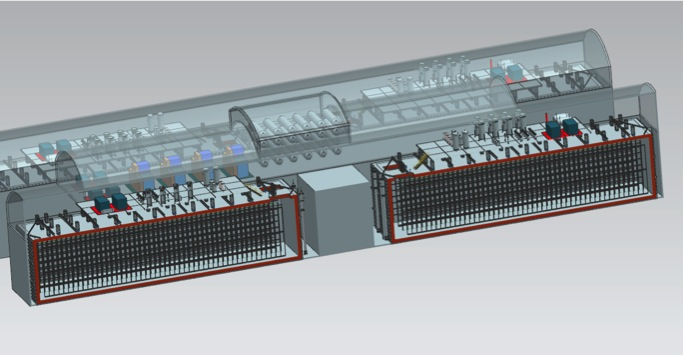
\includegraphics[width=.58\textwidth]{FarDet-3D-SP.jpg}
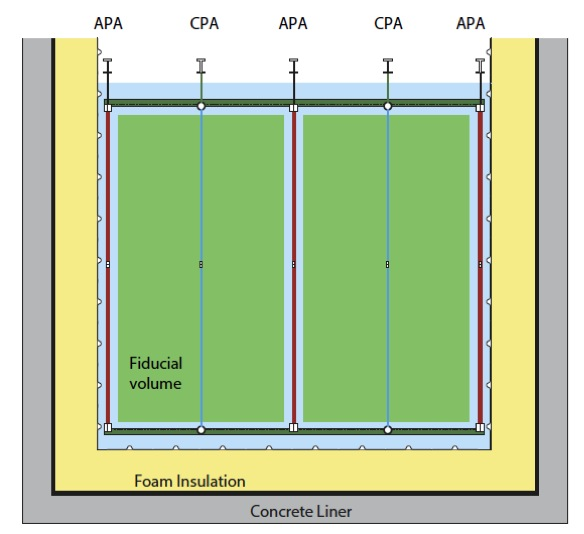
\includegraphics[width=0.38\textwidth]{FarDet-endview-SP.jpg}
\end{center}
\end{minipage}
\end{cdrfigure}
Planning for the conventional facilities calls for construction of the
second cryostat to be completed prior to filling the first so that it
may serve initially as a liquid storage facility.  The detector
technology is expected to improve in the coming years with MicroBooNE,
the SBN program and the CERN neutrino platform.  DUNE's staged program
allows selection of optimal designs for each module as the technology
evolves.


The reference design presented in this chapter and documented in the
project cost and schedule is patterned after the successful ICARUS
experiment, but adapted to the local site requirements at SURF and the
scaled up detector size.  The TPC configuration is shown on the right
in Figure~\ref{fig:FarDet-overview-SP}.  The TPC, described in
Section~\ref{sec:detectors-fd-ref-tpc}, is constructed by placing
alternating high-voltage cathode planes and anode readout planes in a
bath of ultra-pure liquid argon. Particles interacting in the argon
generate electron-ion pairs and scintillation light.

The single-phase design offers the advantage that the charge is
collected directly without gain, enabling precision charge
calibration. However, signal levels are low, requiring the use of cold
electronics (Section~\ref{sec:detectors-fd-ref-ce}). The readout is
based on stereo induction and collection planes, requiring a
deconvolution of the induced signal. A photon detection system
(Section~\ref{sec:detectors-fd-ref-pd}) provides the $t_0$ or event
time for physics processes that are uncorrelated with the LBNF
neutrino beam.
